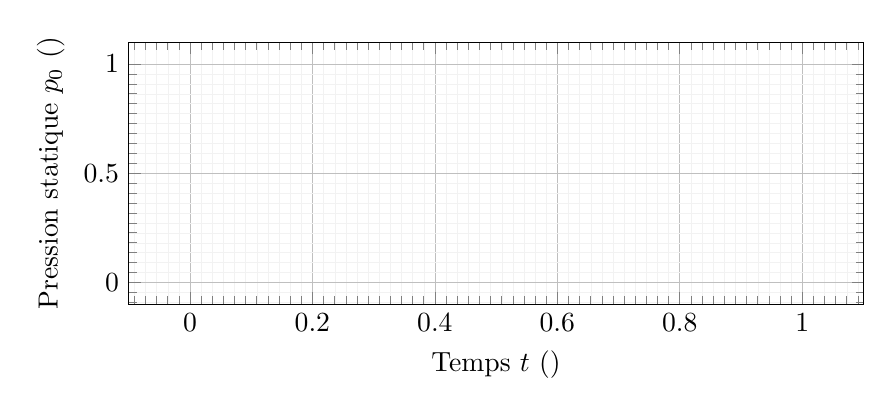
\begin{tikzpicture}
    \def\width{.9*\textwidth};
    \def\height{.45*\width};
    \def\spx{.25cm};
    \def\spy{1.25cm};
    \def\legx{.5cm};
    \def\legy{\legx};
    \def\prop{.45};

    
    \begin{axis}[name=TenuePress,width={\width},height={\height},
    grid=both, minor tick num=10, 
    grid style={line width=.1pt, draw=gray!10},
    major grid style={line width=.2pt,draw=gray!50},
    xlabel={Temps $t$ (\unit{\jour})},
    ylabel={Pression statique $p_0$ (\unit{\pascal})},
%    xmin=0,xmax=75,ymin=0,ymax=.5/1000,
%    xtick={0,25,50,75,100}, ytick={0,1e-4,...,10e-4},
    scaled y ticks = false,
    domain=0:100,
    legend cell align={left},
    legend style = {at={($(1,1)+(-2mm,-2mm)$)},anchor = north east,rounded corners}
    ]
    
%    \addplot[Plasma1, ultra thick] coordinates {(1,1),}

    \end{axis}
\end{tikzpicture}